% !TeX root = ../final.tex
% Revised one-hour lecture script.
% Teaching arc: DESIGN AND EXECUTE EXPERIMENTS.

\chapter{Generating useful chemical data}

\begin{notebox}
  \keypoint{What do you need to learn from this chapter?}
  By the end of this chapter, you should be able to design an experimental dataset for a stated chemical question, distinguish experiment count from information content, decide when endpoints, progress curves, replicates, controls, and negative results are required, identify failure modes in high-throughput experimentation, and choose among parallel batch, continuous-flow, and stopped-flow platforms.
  You should also be able to specify the measurement and provenance needed to make the resulting data interpretable and reusable.
\end{notebox}

% Suggested timing: 0--7 min
\section{More experiments or more information?}

Consider four datasets.

\solution{5.4cm}{%
  \begin{tabular}{p{0.08\linewidth}p{0.80\linewidth}}
    \textbf{A} & 500 measurements from a narrow cluster of closely related ligands.\\[0.35em]
    \textbf{B} & 40 measurements deliberately spanning the steric and electronic ligand space relevant to the project.\\[0.35em]
    \textbf{C} & 1000 endpoint yields measured after 24 hours.\\[0.35em]
    \textbf{D} & 100 complete reaction-progress curves across selected substrate, catalyst, and pH conditions.
  \end{tabular}
}

Which dataset is largest?
Which better tests structural generality?
Which can reveal an induction period, catalyst deactivation, product inhibition, or a change in kinetic regime?

Dataset A contains more rows than B, but it may provide less coverage of the intended chemical space.
Dataset C contains more numerical values than D if each reaction is reduced to one yield, but it has discarded the time-dependent behaviour.
Information content depends on the question.

A titration provides a smaller-scale version of the same lesson.
Ten closely spaced measurements on the flat, saturated part of a binding curve do not define the affinity as well as measurements deliberately distributed across the baseline, transition, and saturation regions.
The informative design depends on the model parameters that must be constrained, not simply on the number of additions.

\solution{3.6cm}{%
  \textbf{Draw two binding experiments.}
  On the first curve, place nearly every point on the saturation plateau.
  On the second, distribute points before, through, and after the transition.
  Which experiment better constrains the midpoint and why?
}

If the objective is rapid screening for a product, a reliable endpoint may be sufficient.
If the objective is to separate competing kinetic models, the reaction profile is part of the evidence.
If the objective is to train a model for new ligand families, deliberate coverage may matter more than repeating measurements in one dense region.

\solution{3.8cm}{%
  \textbf{Complete the sentence for each project:}\\[0.4em]
  ``An informative experiment is one that \ldots''
  \begin{itemize}
    \item finds a productive condition;
    \item distinguishes two kinetic hypotheses;
    \item tests transfer to a new catalyst family;
    \item estimates experimental variability;
    \item exposes a systematic plate or analytical artefact.
  \end{itemize}
}

% Suggested timing: 7--15 min
\section{Design the experiment for the question}

\section{One variable at a time}

A common optimisation strategy in synthetic laboratories is the so-called \keypoint{one-variable-at-a-time} (OVAT) approach.
In this strategy, we change one conditions of the process while holding the others fixed.
The procedure is intuitive, produces plots that are easy to interpret locally, and can be practical when experiments are expensive or difficult to reconfigure.

A problem occurs when the effect of one variable depends on the level of another.
For example, increasing temperature may improve conversion with one base but accelerate decomposition with another.
An OVAT experiment performed at only one base identity cannot reveal the full interaction.
The resulting path can stop at a locally favourable setting while missing a better region elsewhere.

\solution{6.0cm}{%
  \centering
  \resizebox{0.7\linewidth}{!}{%
    \begin{tikzpicture}[
      axis/.style={draw=darkGrey,line width=1.4pt,->,>=Stealth},
      contour/.style={draw=darkBlue,line width=1.1pt},
      path/.style={draw=darkRed,line width=2.3pt,->,>=Stealth},
      point/.style={fill=darkRed,draw=darkRed},
      label/.style={font=\small\sffamily,text=darkGrey,align=center}
    ]
      \draw[axis] (0,0) -- (9,0) node[below] {temperature};
      \draw[axis] (0,0) -- (0,6) node[left,rotate=90] {equivalents};
      \draw[contour] (5.9,3.5) ellipse (3.0 and 2.0);
      \draw[contour] (5.9,3.5) ellipse (2.2 and 1.4);
      \draw[contour] (5.9,3.5) ellipse (1.3 and 0.8);
      \fill[darkGreen] (5.9,3.5) circle (4pt);
      \draw[path] (1.0,1.0) -- (4.2,1.0);
      \draw[path] (4.2,1.0) -- (4.2,3.1);
      \foreach \x/\y in {1.0/1.0,4.2/1.0,4.2/3.1}{\fill[point] (\x,\y) circle (3.4pt);}
      \node[label,text=darkRed] at (2.4,0.55) {OVAT path};
      \node[label,text=darkGreen] at (6.2,4.0) {true optimum};
    \end{tikzpicture}%
  }
}


A conventional one-variable-at-a-time experiment changes one factor while holding the others fixed.
OVAT is useful when we want a local, interpretable perturbation.
For example, changing only catalyst concentration can support a kinetic order measurement when the other conditions are controlled.
It is less effective for mapping interactions across a large optimisation space.

Suppose that temperature improves conversion with base A but accelerates decomposition with base B.
An OVAT path explored only at base A cannot discover that interaction.
It may stop at a locally favourable condition while missing another region.

A factorial design varies several factors systematically.
A simple two-level factorial design can estimate main effects and interactions.
Centre points can reveal curvature that a purely linear response surface would miss.
The fitted response surface remains empirical; it does not become a reaction mechanism merely because the design was systematic.

A framework for a factorial design where several factors are varied to estimate the curvature of the response surface is \keypoint{design-of-experiments} (DoE).
The fitted surface remains empirical, but it can identify influential variables, interactions, and promising regions more efficiently than a sequence of uncoordinated tests.

\solution{6.0cm}{%
  \centering
  \resizebox{0.45\linewidth}{!}{%
  \begin{tikzpicture}[
    axis/.style={draw=darkGrey,line width=1.4pt,->,>=Stealth},
    full/.style={fill=darkBlue,draw=darkBlue},
    centre/.style={fill=darkYellow,draw=darkGrey,line width=1pt},
    label/.style={font=\small\sffamily,text=darkGrey}
  ]
    \draw[axis] (0,0) -- (8,0) node[below] {factor A};
    \draw[axis] (0,0) -- (0,5.5) node[left,rotate=90] {factor B};
    \foreach \x in {1.2,3.7,6.2}{\foreach \y in {1.0,2.7,4.4}{\fill[full] (\x,\y) circle (3.4pt);}}
    \fill[centre] (3.7,2.7) circle (5pt);
    \node[label] at (5.8,5.0) {factorial grid};
    \node[label] at (4.9,2.25) {centre point tests curvature};
  \end{tikzpicture}%
  }
  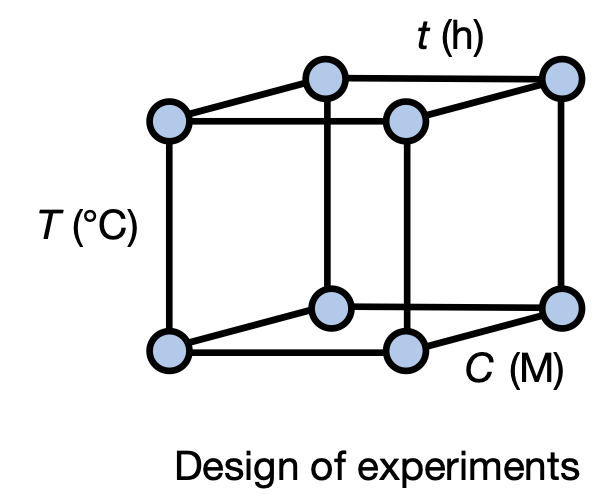
\includegraphics[width=0.45\textwidth]{figures/CH6-doe.png}
}


\solution{5.2cm}{%
  \textbf{Draw two maps of temperature against reagent equivalents.}
  \begin{enumerate}
    \item On the first, draw an OVAT path: change temperature, fix it, then change equivalents.
    \item On the second, mark a factorial design and a centre point.
    \item Add an interaction: the effect of temperature reverses at high equivalents.
  \end{enumerate}
  Which design can expose the interaction without already knowing where it occurs?
}

Chemical-space selection answers a different question.
If the candidates are molecules rather than continuous conditions, descriptors and clustering can select a smaller set that spans the intended representation.
This was the logic behind the catalyst training set in Chapter~5.
Factorial designs, chemical-space sampling, kinetic perturbations, and replication are therefore complementary tools rather than competing brands of experimental design.

Negative outcomes are also designed observations.
A reaction that produces no detectable product can constrain a model, but only if the experiment was executed correctly and the analytical method was capable of detecting the expected product.
A failed injection is not a negative chemical result.

% Suggested timing: 15--23 min
\section{Automation changes scale, not scientific validity}

Parallel high-throughput experimentation uses arrays of wells or vessels to perform coordinated experiments.
Liquid and solid handlers can dispense reagents, while heating, shaking, sampling, and analysis can be scheduled reproducibly.
Miniaturisation reduces material use and permits systematic exploration that would be impractical manually.

The scientific benefit is not simply that a robot is fast.
Automation can execute the same experimental design repeatedly and record operations at a scale where systematic sampling becomes possible.
It can also reproduce a mistake with exceptional consistency.

\solution{5.0cm}{%
  \textbf{Spot the failure modes in a 96-well plate.}
  \begin{itemize}
    \item evaporation is greatest at the plate edge;
    \item a suspension settles before later wells are dispensed;
    \item one stock solution has the wrong concentration;
    \item mixing is inadequate in the highest-viscosity wells;
    \item the autosampler drifts over the analytical sequence;
    \item one substrate class is integrated using the wrong chromatographic peak.
  \end{itemize}
  For each problem, decide whether randomisation, controls, calibration, replication, or a redesigned procedure would expose it.
}

A plate layout is part of the design.
Blanks expose contamination.
Standards monitor measurement and instrument drift.
Positive controls show whether the campaign remains capable of producing a known response.
Replicates estimate variation.
Randomisation separates a chemical trend from a spatial or temporal trend.
None of these controls can rescue an analytical method that measures the wrong species.

\begin{warningbox}
  \keypoint{Automation amplifies the experimental design.}
  It can amplify informative perturbations and reproducible measurement, or amplify systematic dosing, mixing, sampling, and analytical errors.
\end{warningbox}

% Suggested timing: 23--30 min
\section{Measurement is part of the experiment}

An automated reaction is not complete when heating ends.
The reported value is produced by a chain:

\solution{4.0cm}{%
  \centering
  reaction $\longrightarrow$ sampling $\longrightarrow$ quench $\longrightarrow$ dilution\\[0.6em]
  $\longrightarrow$ transfer $\longrightarrow$ measurement $\longrightarrow$ peak assignment\\[0.6em]
  $\longrightarrow$ processing $\longrightarrow$ quality control $\longrightarrow$ recorded value
}

Every step can change the sample or introduce uncertainty.
A slow quench can allow the reaction to continue.
Evaporation can alter concentration.
A transfer can lose a precipitated product.
An internal standard can degrade.
Peak integration can fail systematically for one substrate family.

Chromatography can separate mixture components.
Mass spectrometry can support molecular-formula or mass assignments.
NMR can report composition and structure.
Optical spectroscopy can provide rapid, time-resolved measurements.
No method answers every question.
Orthogonal methods are valuable when an automated decision must distinguish conversion, identity, purity, topology, and function.

\solution{3.8cm}{%
  A robot executes 384 reactions perfectly, but the LC method systematically under-integrates one product class.\\[0.6em]
  \textbf{Do we have a high-quality dataset?} Explain why experimental execution and measurement validity are separate requirements.
}

The label ``no product'' should be reserved for a sample that passed the relevant execution and analytical checks.
A missing injection, saturated detector, failed integration, ambiguous mass signal, and genuine negative reaction should have different status codes.
Collapsing them all to numerical zero destroys information.

% Suggested timing: 30--38 min
\section{Case study: systematic cage discovery}

Greenaway and co-workers fused computational screening with robotic synthesis for 78 precursor combinations formed from three tritopic amines and 26 aldehydes.\mcite{Greenaway2018}
The experimental matrix recorded clean cage formation, partial formation, and negative outcomes.
Thirty-three combinations produced cages cleanly, and the campaign exposed unexpected doubly bridged, triply interlocked cage catenanes.

\begin{figure}[htbp]
  \centering
  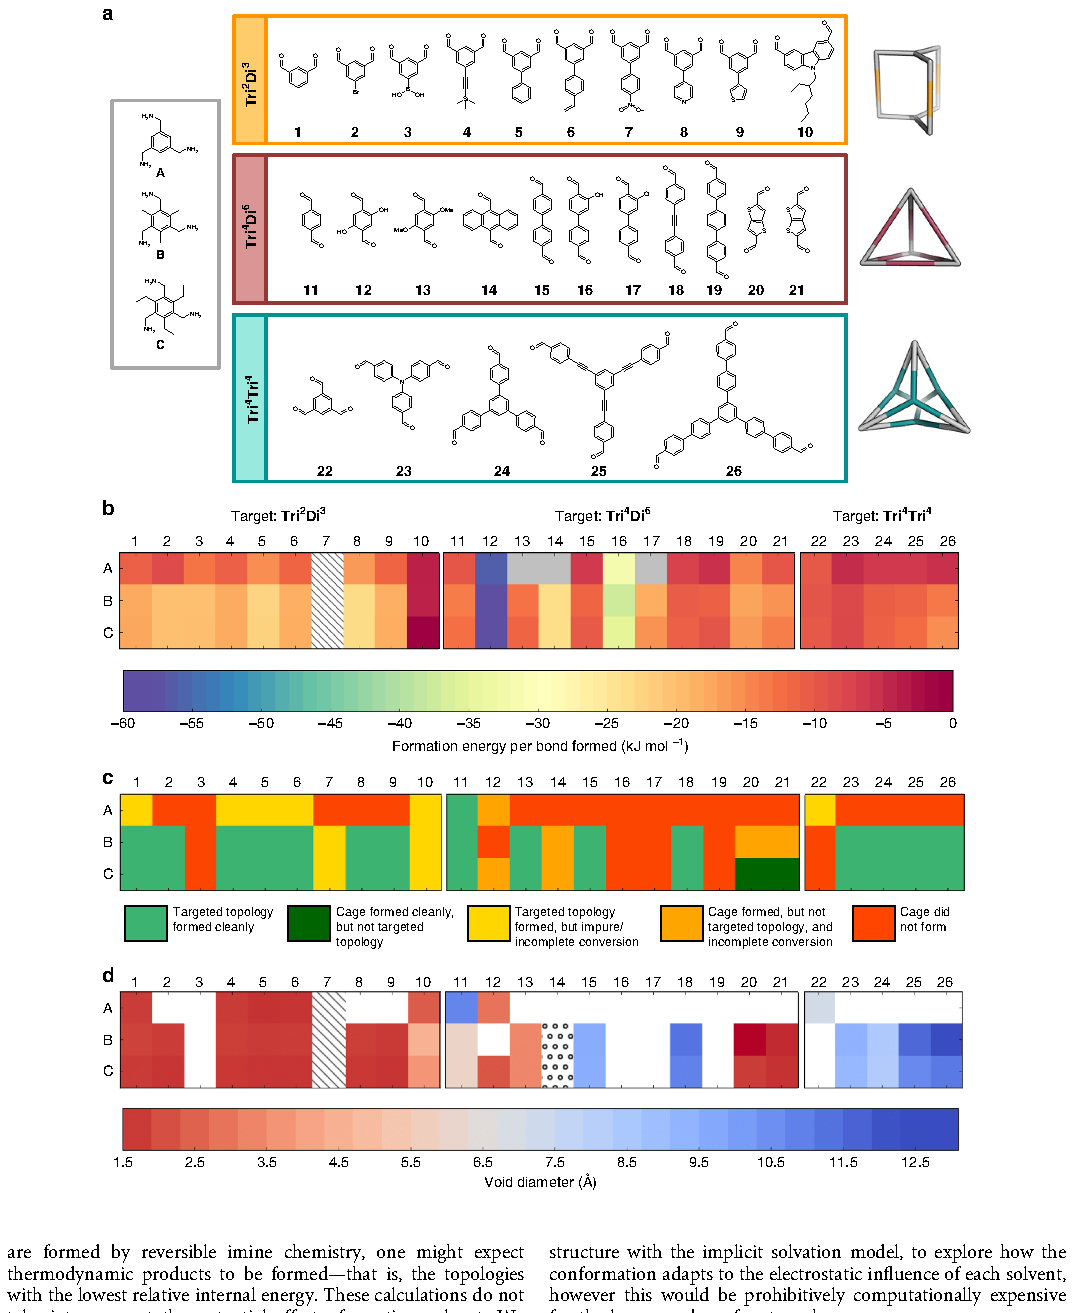
\includegraphics[width=\textwidth,height=0.72\textheight,keepaspectratio]{figures/chapter07-generate/01-greenaway-cage-screen-matrix-fig3.pdf}
  \caption{Precursor combinations, target cage topologies, computational results, and experimental outcomes from a systematic cage screen. Negative and partial outcomes give the successful cages their context. Reproduced from Greenaway \textit{et al.}, \textit{Nature Communications} (2018), Fig.~3.}
  \label{fig7-greenaway-matrix}
\end{figure}

Why is the complete matrix more useful than a paper containing only the 33 successes?
The failed and partial reactions test the computational predictions, identify unreliable precursor families, and reveal the boundary of the synthetic strategy.
The unexpected topology becomes interpretable against an internally comparable background rather than as an isolated curiosity.

\solution{4.2cm}{%
  \textbf{Annotate the Greenaway screening matrix.}
  \begin{itemize}
    \item use different marks for clean cage, partial formation, and no cage;
    \item outline one complete precursor row or column;
    \item circle the unexpected catenane outcome;
    \item write what would be lost if only successful isolated cages were retained.
  \end{itemize}
}

Basford and co-workers expanded automated imine-cage discovery to 366 condensation reactions and automated substantial parts of synthesis, sample preparation, characterisation, and analysis.\mcite{Basford2024}
Turbidity, NMR, and high-resolution mass spectrometry answer different questions.
Turbidity can indicate precipitation or heterogeneous behaviour; NMR can report conversion and mixture composition; mass spectrometry can support assignments of cage stoichiometry.
Together they provide more defensible outcome labels than one signal alone.

The study linked experiments to a much larger computed set of hypothetical structures and pore properties, and deposited experiment maps, code, and raw data.
This is important because a reusable campaign consists not only of a result table but also of the procedures and processing that created those labels.

\solution{3.7cm}{%
  \textbf{Build an evidence table.} For each method---turbidity, NMR, and high-resolution MS---write:
  \begin{enumerate}
    \item what it measures directly;
    \item what chemical conclusion it can support;
    \item what ambiguity remains.
  \end{enumerate}
}

Shields and co-workers used low-cost conformational calculations together with semi-automated high-throughput crystallisation for an amide-linked organic cage.\mcite{ShieldsCage2024}
The calculations identified several accessible cage conformers with different internal acid--acid distances.
The crystallisation screen then trapped all five predicted stable conformers in experimentally determined solid-state structures.

\begin{figure}[htbp]
  \centering
  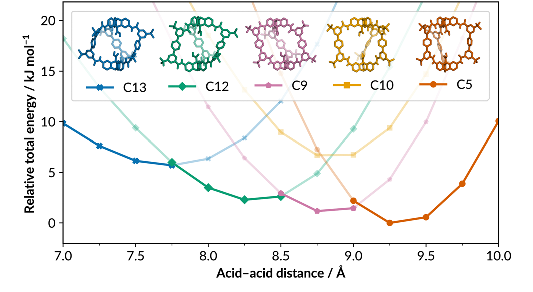
\includegraphics[width=\textwidth,height=0.46\textheight,keepaspectratio]{figures/chapter07-generate/02-shields-cage-computed-conformers-fig2.pdf}
  \caption{The five lowest-energy calculated conformers used to frame the crystallisation search. Reproduced from Shields \textit{et al.}, \textit{Chemical Communications} (2024), Fig.~2.}
  \label{fig7-shields-computed}
\end{figure}\begin{figure}[htbp]
  \centering
  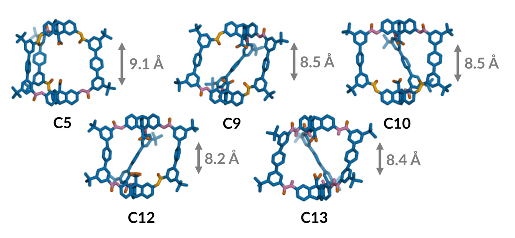
\includegraphics[width=\textwidth,height=0.42\textheight,keepaspectratio]{figures/chapter07-generate/03-shields-cage-observed-conformers-fig3.pdf}
  \caption{Five cage conformations observed experimentally in the solid state. The screen connects predicted flexibility to structures trapped under crystallisation conditions. Reproduced from Shields \textit{et al.}, \textit{Chemical Communications} (2024), Fig.~3.}
  \label{fig7-shields-observed}
\end{figure}

This workflow is systematic and automated, but it is not autonomous in the sense used in Chapter~8.
The measurements did not select the next crystallisation condition during the demonstrated campaign.
The example therefore provides a useful boundary: a broad programmable search can be scientifically powerful without making adaptive decisions.

\solution{3.4cm}{%
  \textbf{Annotate the cage-crystallisation figure.}
  Link each calculated conformer in Fig.~\ref{fig7-shields-computed} to the corresponding experimental solid-state structure in Fig.~\ref{fig7-shields-observed}.
  Mark the fixed experimental campaign and identify where a feedback arrow would have to be added to make the search adaptive.
}

% Suggested timing: 38--46 min
\section{Case study: high-throughput kinetics preserves mechanism}

Kuffer and Mayer combined liquid-handling robotics with continuous UV monitoring to study acid- and base-catalysed addition of urea to carbonyl compounds in water.\mcite{KufferMayer2026}
The campaign produced a consistent dataset of 6889 rate constants.
The important point is not merely the number.
Each rate constant came from a kinetic trace collected across a deliberately varied multiparameter space.

\begin{figure}[htbp]
  \centering
  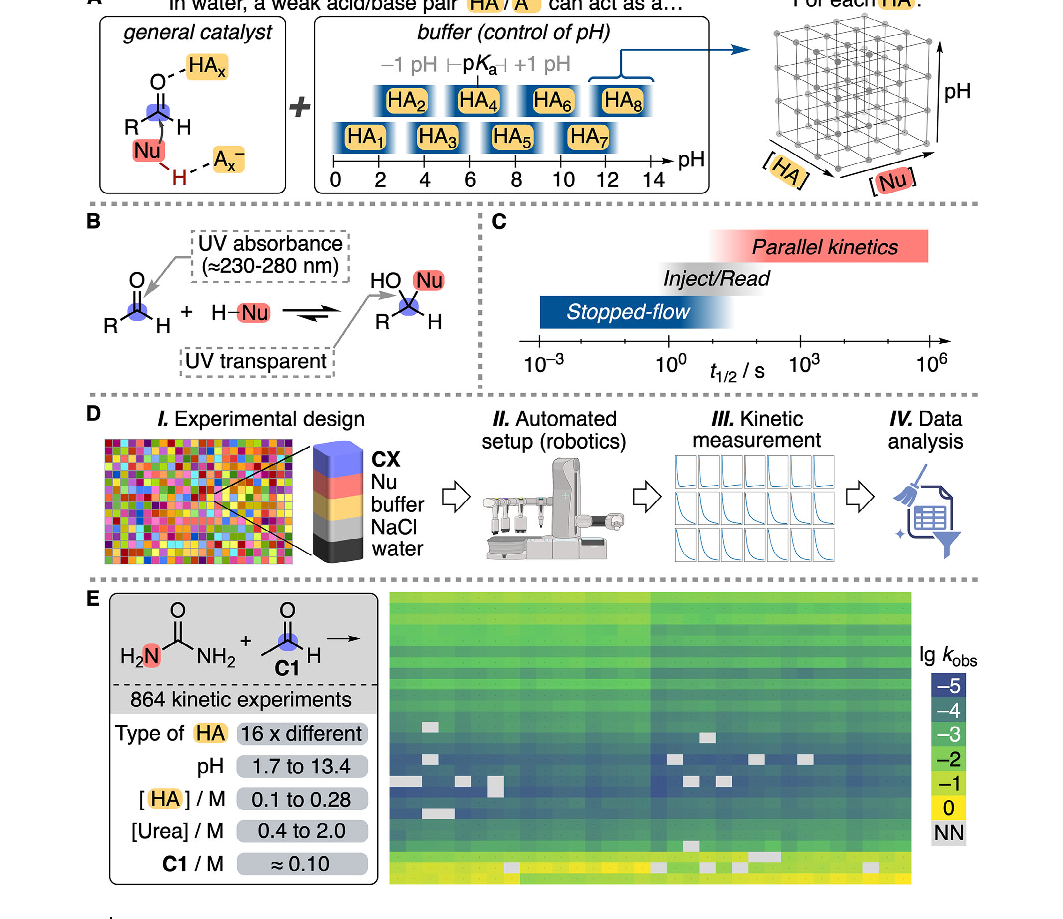
\includegraphics[width=\textwidth,height=0.70\textheight,keepaspectratio]{figures/chapter07-generate/04-kuffer-high-throughput-kinetics-workflow-fig3.pdf}
  \caption{High-throughput kinetic workflow from combinatorial buffer/pH design through automated preparation, continuous UV measurement, and kinetic fitting. Reproduced from Kuffer \textit{et al.}, \textit{Angewandte Chemie International Edition} (2026), Fig.~3.}
  \label{fig7-kuffer-workflow}
\end{figure}

\solution{4.5cm}{%
  \textbf{Follow one experiment from liquid handling to a fitted rate constant.}
  \begin{itemize}
    \item Mark the controlled inputs: substrate, pH, buffer identity, and buffer concentration.
    \item Circle the raw observable and write its units.
    \item Draw the processing arrow from the UV trace to $k_{\mathrm{obs}}$.
    \item Cross out the information that would disappear if only a final absorbance were stored.
  \end{itemize}
}

A measured rate in water can contain contributions from several pathways: uncatalysed background reaction, specific acid catalysis, specific base catalysis, and general acid or base catalysis.
Those contributions have different dependences on pH, buffer identity, buffer concentration, and substrate structure.
Treating the observed rate as one undifferentiated response can hide changes in the dominant mechanism.

\begin{figure}[htbp]
  \centering
  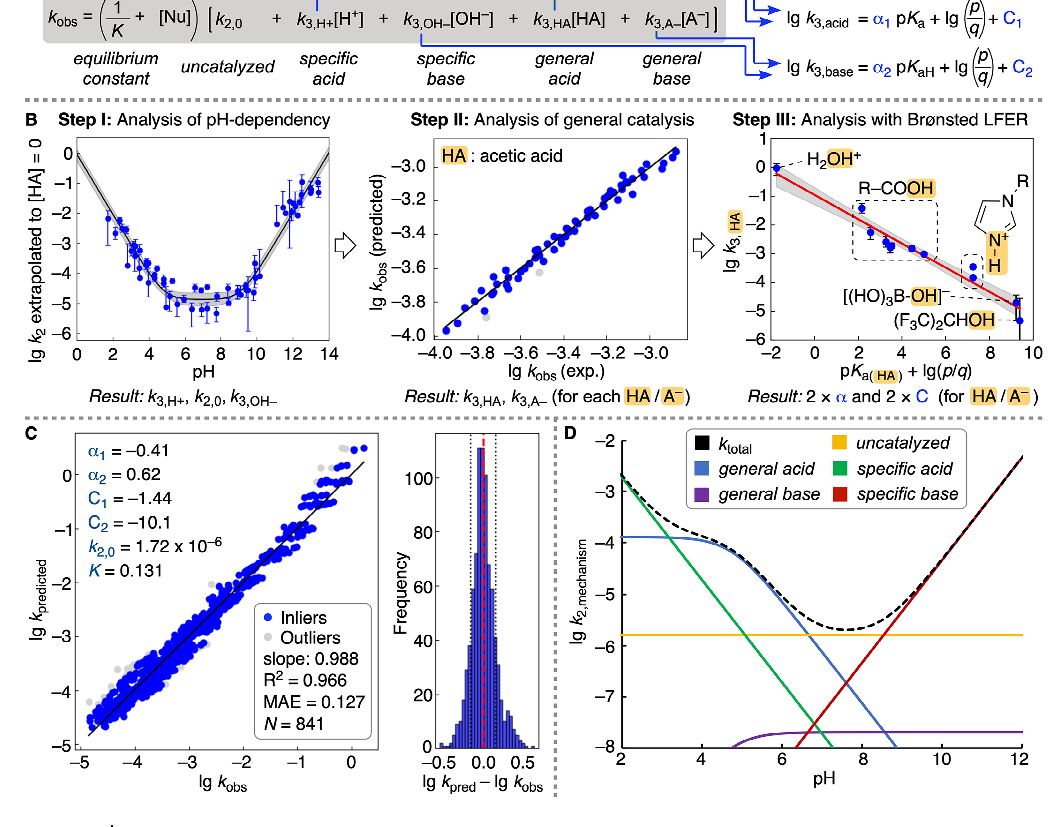
\includegraphics[width=\textwidth,height=0.68\textheight,keepaspectratio]{figures/chapter07-generate/05-kuffer-mechanistic-rate-model-fig4.pdf}
  \caption{Mechanistic decomposition of observed rates into background, specific acid/base, and general acid/base contributions. Reproduced from Kuffer \textit{et al.}, \textit{Angewandte Chemie International Edition} (2026), Fig.~4.}
  \label{fig7-kuffer-mechanism}
\end{figure}

\solution{4.3cm}{%
  \textbf{Annotate the rate model rather than copying it.}
  \begin{itemize}
    \item Use different colours for specific acid/base and general acid/base pathways.
    \item Mark which perturbation isolates pH dependence and which tests buffer catalysis.
    \item Predict how the pH--rate profile changes when the dominant pathway changes.
  \end{itemize}
}

The mechanism-guided model separates pathway contributions and predicts absolute rate constants for selected carbonyl compounds and conditions.
A complementary supervised machine-learning model can predict across a broader substrate set.
The two approaches answer related but distinct questions: one imposes mechanistic structure; the other learns predictive relationships from descriptors and observations.

\begin{figure}[htbp]
  \centering
  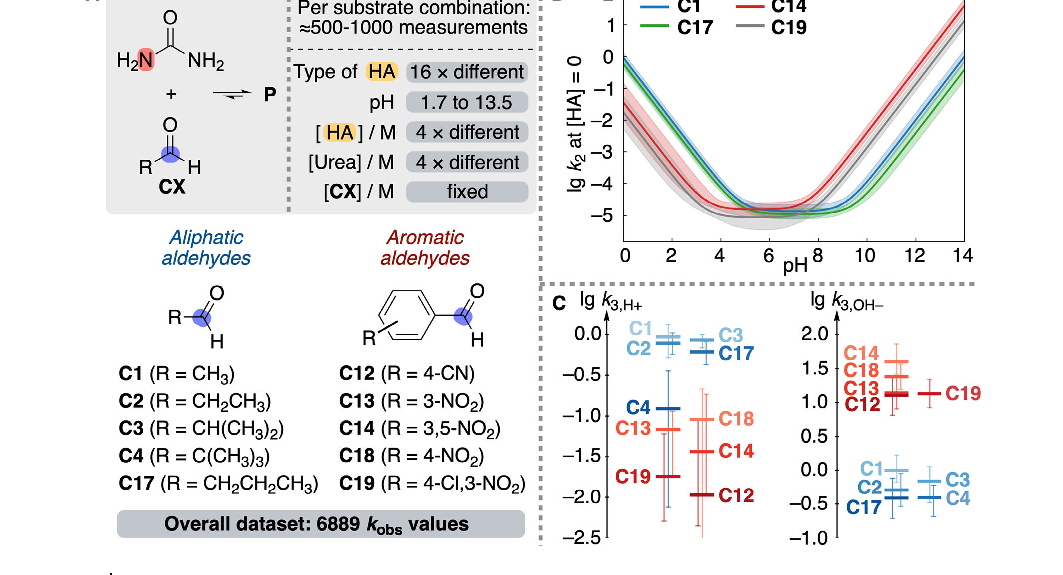
\includegraphics[width=\textwidth,height=0.58\textheight,keepaspectratio]{figures/chapter07-generate/06-kuffer-kinetic-dataset-fig5.pdf}
  \caption{The aldehyde set, fitted pH--rate profiles, and relative reactivities that make up the mechanistically resolved kinetic dataset. Reproduced from Kuffer \textit{et al.}, \textit{Angewandte Chemie International Edition} (2026), Fig.~5.}
  \label{fig7-kuffer-dataset}
\end{figure}

\solution{3.8cm}{%
  \textbf{Read the dataset as a set of curves, not a table of endpoints.}
  \begin{itemize}
    \item Mark the regions dominated by acid and base catalysis.
    \item Compare two aldehydes and write which observation supports a genuine reactivity difference.
    \item Circle where uncertainty is largest and propose one additional measurement.
  \end{itemize}
}\begin{figure}[htbp]
  \centering
  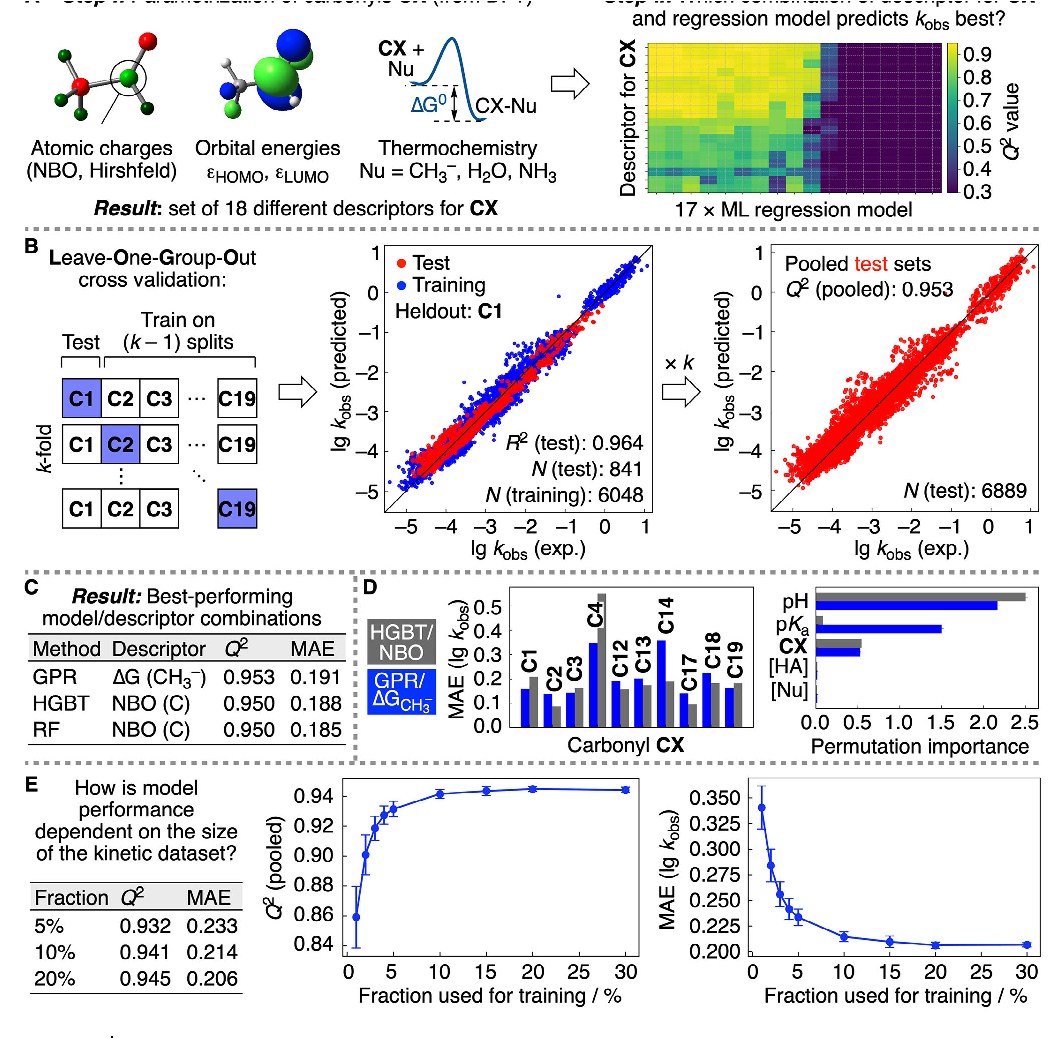
\includegraphics[width=\textwidth,height=0.70\textheight,keepaspectratio]{figures/chapter07-generate/07-kuffer-ml-reactivity-prediction-fig6.pdf}
  \caption{Descriptor/model comparison, leave-one-group-out validation, and prospective reactivity prediction from the kinetic dataset. Reproduced from Kuffer \textit{et al.}, \textit{Angewandte Chemie International Edition} (2026), Fig.~6.}
  \label{fig7-kuffer-ml}
\end{figure}

\solution{4.0cm}{%
  \textbf{Separate the predictive and mechanistic claims.}
  \begin{itemize}
    \item Mark the validation design that tests transfer to a withheld carbonyl compound.
    \item Circle the prospective prediction and the experiment that checks it.
    \item Write one conclusion supported by prediction and one that still requires mechanistic evidence.
  \end{itemize}
}

\solution{4.8cm}{%
  \textbf{Now connect Figs.~\ref{fig7-kuffer-workflow}--\ref{fig7-kuffer-ml} into one evidence chain.}
  \begin{itemize}
    \item mark the raw observable (absorbance versus time);
    \item mark the derived quantity (rate constant);
    \item add the variables that change pathway contributions: pH, buffer, and substrate;
    \item identify where an endpoint-only workflow would discard information.
  \end{itemize}
}

Suppose that the experimental budget allows 1000 measurements.
One option is 1000 endpoint absorbances under many conditions.
Another is a smaller number of complete traces that can be fitted and compared across catalytic regimes.
The correct choice depends on whether we seek a hit, a predictive rate model, or a mechanistic decomposition.
This case shows that automation does not replace physical-organic chemistry.
It allows controlled perturbation, kinetic measurement, model comparison, and mechanism testing at scale.

\begin{conceptbox}
  \keypoint{Throughput is most valuable when the measurement retains the information required by the question.}
  A large endpoint screen and a dense kinetic dataset are not interchangeable, even if they use the same robot.
\end{conceptbox}

% Suggested timing: 46--54 min
\section{Choose the experimental platform}

Parallel batch, continuous flow, and stopped flow organise time and material differently.
The architecture should follow the chemical and analytical problem.

\subsection{Parallel batch}

A plate can run many categorical combinations simultaneously.
It is well suited to libraries of catalysts, ligands, substrates, or reagents and to reactions with compatible heating and mixing requirements.
Well-to-well evaporation, dispensing limits, solids, sealing, and spatial effects require deliberate controls.

\subsection{Continuous flow}

High-throughput experimentation does not require a single type of reactor. In the examples above, many reactions are carried out in parallel, for example in well plates. That is extremely useful when we want to compare many combinations of substrates, catalysts, or additives under similar conditions. However, some experiments are awkward to perform in a plate.

Consider a reaction that we want to study over a range of temperatures, including temperatures above the normal boiling point of the solvent. We may also want tight control of mixing, reaction time, and automated sampling for analysis. In that situation, rather than running many small batch reactions in parallel, we can move reaction mixtures continuously through a controlled reactor.

\solution{5.8cm}{
\begin{center}
\begin{tikzpicture}[
    >=latex,
    node distance=8mm and 10mm,
    every node/.style={font=\small},
    box/.style={draw, rounded corners=2pt, minimum height=8mm, minimum width=19mm, align=center},
    line/.style={->, thick}
]
\node[box] (a) {stock A};
\node[box, below=of a] (b) {stock B};
\node[box, right=of $(a)!0.5!(b)$] (pump) {pumps};
\node[box, right=of pump] (mix) {mixer};
\node[box, right=of mix, minimum width=31mm] (reactor) {heated reactor};
\node[box, right=of reactor, minimum width=25mm] (bpr) {back-pressure\\regulator};
\node[box, right=of bpr] (analysis) {analysis};

\draw[line] (a.east) -- (pump.west);
\draw[line] (b.east) -- (pump.west);
\draw[line] (pump) -- (mix);
\draw[line] (mix) -- (reactor);
\draw[line] (reactor) -- (bpr);
\draw[line] (bpr) -- (analysis);

\node[below=7mm of reactor, align=center] (q) {What can we control?};
\draw[->, thin] (q.north) -- (reactor.south);
\node[below=2mm of q, align=center] {composition \quad flow rate \quad temperature \\ pressure \quad reaction time};
\end{tikzpicture}
\end{center}
}

The important idea is not that ``flow'' is intrinsically better than batch chemistry. It is a different experimental architecture. Reagents are delivered at controlled rates, mixed, passed through a reactor under defined conditions, and then sent onwards for analysis or collection. The experiment is therefore particularly amenable to systematic changes in conditions and to computer control.

A few consequences are useful for us here. Flow reactors can be pressurised, so reactions can be performed above the normal boiling point of the solvent. Small reactor volumes can provide efficient heat transfer and rapid mixing. Conditions can also be changed programmatically, and the reactor outlet can be connected directly to analytical instruments. These features make flow useful when the aim is to generate reproducible reaction data across a controlled experimental space.

In a batch flask, we usually specify how long the reaction is left before sampling or work-up. In flow, the equivalent quantity is set by how quickly the reaction mixture travels through a reactor of known volume. For an idealised reactor,
\[
    \tau \approx \frac{V}{Q},
\]
where $V$ is the reactor volume and $Q$ is the total volumetric flow rate. We will not treat reactor engineering in detail here; the useful point is simply that reaction time becomes another experimentally programmable variable.

\subsection{What are the limitations of continuous flow?}

The same architecture also creates practical constraints. Reagents must be delivered reliably through pumps and tubing. Solids, precipitation, and viscous mixtures can cause blockages or fouling. Changing from one set of conditions to another is not instantaneous because material already present in the tubing and reactor must first pass through the system. Long reaction times may require larger reactor volumes or low flow rates. Cleaning and carry-over between experiments can also become important when many different reactions are run automatically.

There is a further issue when material is valuable. In a conventional continuous-flow experiment, reagents continue to move through the reactor while the system operates. For library synthesis or reaction screening, where we may have only small quantities of each substrate, continually pumping material can therefore be wasteful.

This motivates an intermediate approach.

\subsection{Stopped-flow experimentation}

In stopped-flow synthesis, a defined segment of reaction mixture is pumped into the reactor and then the flow is stopped. The mixture reacts for the chosen time without further reagent being consumed. Flow is then restarted to move the reaction mixture to analysis and introduce the next experiment.

\solution{5.3cm}{
\begin{center}
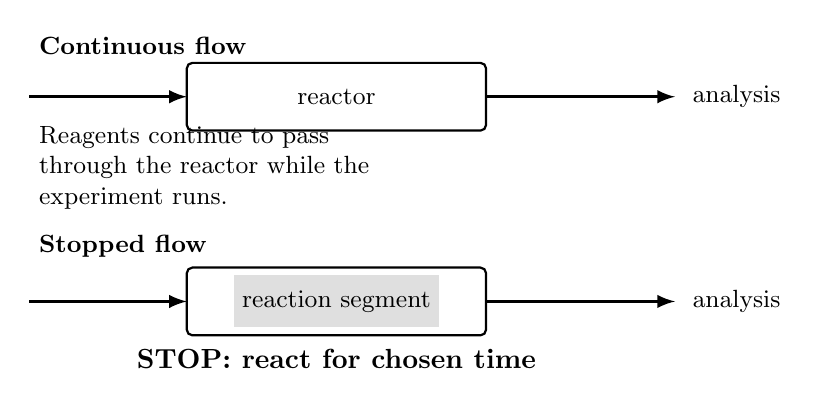
\begin{tikzpicture}[>=latex, every node/.style={font=\small}]
% continuous
\node[anchor=west, font=\small\bfseries] at (0,2.8) {Continuous flow};
\draw[->, very thick] (0,2.15) -- (2.0,2.15);
\draw[thick, rounded corners=2pt] (2.0,1.72) rectangle (5.8,2.58);
\node at (3.9,2.15) {reactor};
\draw[->, very thick] (5.8,2.15) -- (8.2,2.15);
\node[anchor=west] at (8.3,2.15) {analysis};
\node[anchor=west, text width=4.4cm] at (0,1.25) {Reagents continue to pass through the reactor while the experiment runs.};

% stopped
\node[anchor=west, font=\small\bfseries] at (0,0.25) {Stopped flow};
\draw[->, very thick] (0,-0.45) -- (2.0,-0.45);
\draw[thick, rounded corners=2pt] (2.0,-0.88) rectangle (5.8,-0.02);
\fill[gray!25] (2.6,-0.78) rectangle (5.2,-0.12);
\node at (3.9,-0.45) {reaction segment};
\draw[->, very thick] (5.8,-0.45) -- (8.2,-0.45);
\node[anchor=west] at (8.3,-0.45) {analysis};
\node[font=\bfseries] at (3.9,-1.18) {STOP: react for chosen time};
\end{tikzpicture}
\end{center}
}

Avila and co-workers used this idea for automated library synthesis. Their platform combined automated reagent delivery, a stopped-flow reactor, and at-line analysis. They performed 900 reactions in 192 hours, while estimating that the stopped-flow strategy used only about 10\% of the reagents and solvents required for an equivalent fully continuous approach. The resulting experimental data were then used to train a neural-network model and guide further experiments.

This example is useful because it shows that the choice of experimental platform is part of experimental design. Parallel batch, continuous flow, and stopped flow are not competing technologies with a single winner. Each makes different compromises between throughput, reaction conditions, material consumption, and ease of automation.


\begin{figure}[htbp]
  \centering
  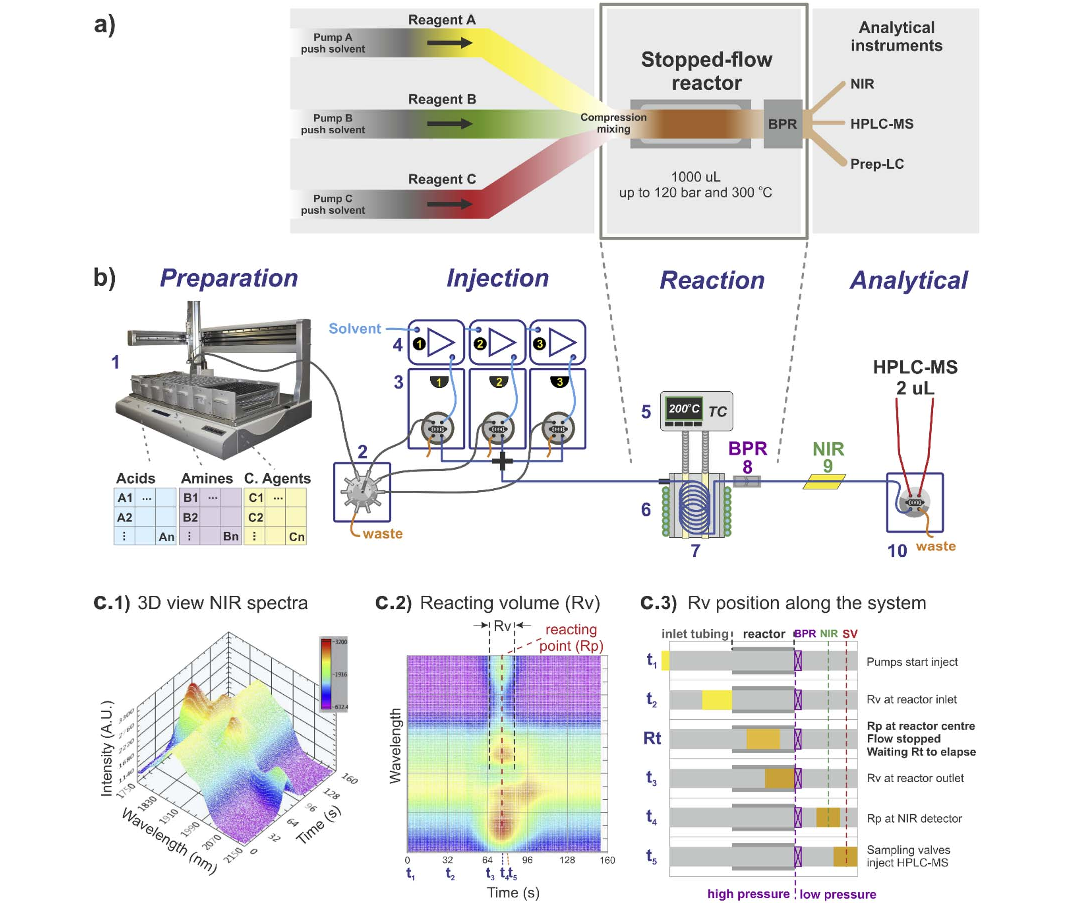
\includegraphics[width=\textwidth,height=0.70\textheight,keepaspectratio]{figures/chapter07-generate/08-avila-stopped-flow-platform-fig1.pdf}
  \caption{Stopped-flow reactor concept and its integration with liquid handling, pumps, sampling loops, temperature control, and analysis. Reproduced from Avila \textit{et al.}, \textit{Chemical Science} (2022), Fig.~1.}
  \label{fig7-avila-stopped-flow}
\end{figure}

\solution{4.2cm}{%
  \textbf{Annotate material and time in the stopped-flow platform.}
  \begin{itemize}
    \item Trace one reaction segment from preparation to analysis.
    \item Mark when flow stops, when reaction time begins and ends, and where carry-over could occur.
    \item Compare the material wasted here with the material needed to establish steady state in continuous flow.
  \end{itemize}
}
The architecture combines access to elevated temperature and pressure with flexible reaction times while avoiding the material cost of maintaining every condition at continuous steady state.

The study performed hundreds of reactions and generated standardised observations for a feed-forward neural network.
This is a useful middle ground between parallel batch and conventional continuous flow: serial reactor hardware can run a library without wasting large volumes during steady-state establishment.
It also makes the trade-off visible.
The system gains flexibility and material efficiency, but each segment still requires reliable transport, timing, cleaning, and analysis.

\solution{4.5cm}{%
  \textbf{Choose a platform for each problem.}
  \begin{enumerate}
    \item Screen 96 combinations of solid-supported catalysts and four solvents.
    \item Vary temperature, residence time, and equivalents with rapid inline analysis.
    \item Build a small-molecule library at elevated pressure where each reaction requires a different hold time and material is scarce.
  \end{enumerate}
  Compare parallel batch, continuous flow, and stopped flow; justify the decision chemically rather than technologically.
}

Flow is not automatically superior to batch.
A hybrid platform may prepare samples in parallel, react them serially, and analyse them on a shared instrument.
The relevant bottleneck may be dosing, residence time, separation, or measurement rather than the reaction itself.

% Suggested timing: 54--59 min
\section{Practical FAIR chemical data}

The FAIR principles describe data that are \keypoint{findable, accessible, interoperable, and reusable}.\mcite{Wilkinson2016}
In chemical experiments, reusability requires more than a table of yields.
The record should identify materials and structures, quantities and units, conditions and timing, and any other relevant \textit{metadata}.
Sensitive or proprietary data can remain access controlled while still ensure interoperability using persistent identifiers and datatype definitions (\textit{schemas}).
Accessibility means that authorised users and machines can retrieve the data and its metadata through a clear procedure.
Importantly, \keypoint{unsuccessful experiments are also part of the scientific record}.
While there are plenty of large-scale resources of FAIR scientific data, for wider adoption of our own experimental work we should strive to follow FAIR principles even for smaller datasets.
Repositories such as Zenodo help ensure findability and accessibility.

\solution{10cm}{%
  \centering
  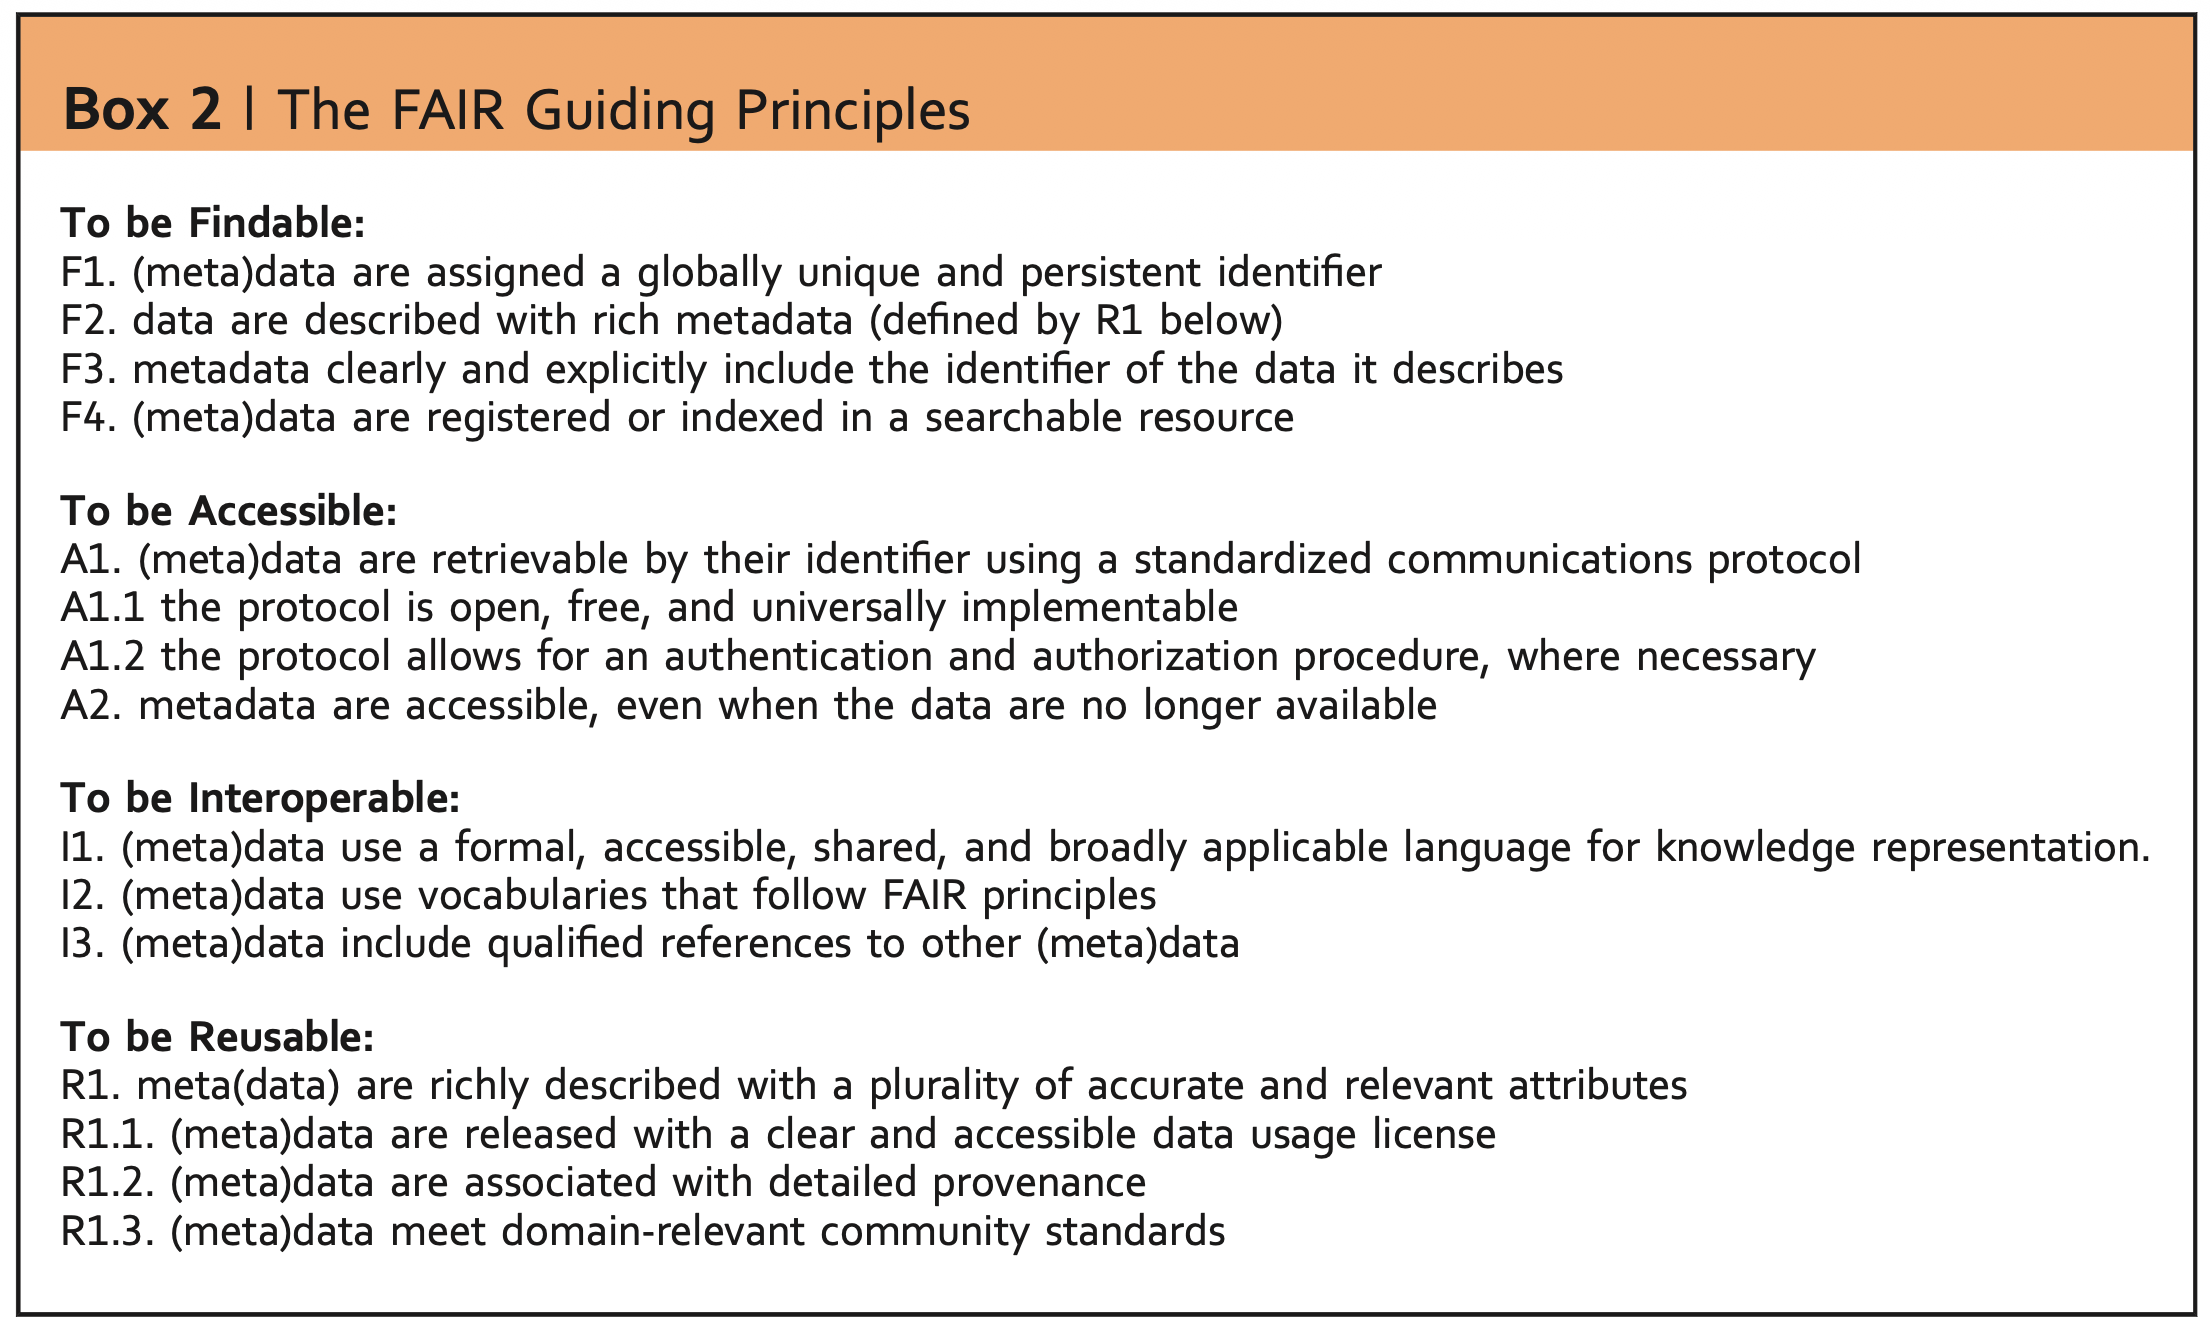
\includegraphics[width=\textwidth]{figures/CH6-fair.png}
}

Compare:

\solution{5.2cm}{%
  \begin{tabular}{p{0.10\linewidth}p{0.78\linewidth}}
    \textbf{A} & substrate = 4a; solvent = THF; yield = 73.\\[0.5em]
    \textbf{B} & structure and persistent identifier; reagent source and batch; concentrations and units; addition order; vessel; atmosphere; temperature profile; timestamps; analytical method and calibration; raw data; processing version; result; uncertainty; QC status; and explicit failure state.
  \end{tabular}
}

Record A may be intelligible to the person who performed the reaction yesterday.
It is not enough for another group, a future student, or an automated workflow to reproduce and interpret the result.
Record B connects the numerical response to the material, procedure, measurement, and processing that produced it.

\solution{3.8cm}{%
  \textbf{Design a failure-state vocabulary.} Distinguish at least:
  \begin{itemize}
    \item valid chemical negative;
    \item reaction-execution failure;
    \item analytical failure;
    \item processing failure;
    \item sample not measured;
    \item result rejected by quality control.
  \end{itemize}
}

A reusable record includes provenance: which raw signal, calibration, processing script, and decision produced the final value.
Without provenance, a result can be impossible to audit even when the final table looks tidy.
This becomes essential in Chapter~8 because an automated system may use one accepted value immediately to choose the next experiment.

% Suggested timing: 59--60 min
\section{Summary}

Experiment count and chemical information are not equivalent.
Experimental design should follow the scientific question: OVAT isolates local effects, factorial designs expose interactions, chemical-space selection tests structural coverage, progress curves preserve kinetic behaviour, and replicates estimate variability.
Automation enables systematic execution at scale but also reproduces systematic failure.
Measurement, quality control, and explicit failure states are part of the dataset.
The Greenaway and Basford cage studies show the value of complete matrices, negative outcomes, orthogonal analysis, and reusable workflows.
The Shields cage study distinguishes a broad automated campaign from an adaptive one.
The Kuffer--Mayer study shows how high-throughput kinetic traces can support mechanistic pathway separation rather than merely producing more endpoints.
Parallel batch, continuous flow, and stopped flow should be selected according to the variables, material constraints, transport, and analytical task.
FAIR data connect structures and conditions to raw measurements, processing, provenance, and quality status.
The next chapter begins when these reliable measurements change the decision about which experiment happens next.
